\begin{frame}{Clinical Artifact 5: Utility--Fairness Frontier}
\begin{center}
\IfFileExists{../analysis_artifacts/fig5_utility_fairness_frontier.pdf}{\includegraphics[width=0.86\textwidth,height=0.62\textheight,keepaspectratio]{../analysis_artifacts/fig5_utility_fairness_frontier.pdf}}{%
\IfFileExists{../analysis_artifacts/fig5_utility_fairness_frontier.png}{\includegraphics[width=0.86\textwidth,height=0.62\textheight,keepaspectratio]{../analysis_artifacts/fig5_utility_fairness_frontier.png}}{%
\IfFileExists{../analysis_artifacts/utility_fairness_frontier.pdf}{\includegraphics[width=0.86\textwidth,height=0.62\textheight,keepaspectratio]{../analysis_artifacts/utility_fairness_frontier.pdf}}{%
\begin{tikzpicture}
\begin{axis}[width=0.8\textwidth,height=0.55\textheight,xlabel={Utility / efficiency index},ylabel={Remaining disparity gap (pp)},xmin=68,xmax=96,ymin=0,ymax=30,grid=both]
\addplot+[mark=*] coordinates {(72,25) (84,18) (88,6) (91,2)};
\node at (axis cs:72,25) [anchor=south west,font=\scriptsize] {Baseline};
\node at (axis cs:84,18) [anchor=south west,font=\scriptsize] {Utility-only CMAB};
\node at (axis cs:88,6) [anchor=south west,font=\scriptsize] {Fair CMAB};
\node at (axis cs:91,2) [anchor=south west,font=\scriptsize] {EQUITAS};
\end{axis}
\end{tikzpicture}}}}
\end{center}
\small The target region is high utility with low remaining disparity. The question is how much performance is preserved when context is handled correctly.
\end{frame}
